\documentclass[11pt,twocolumn]{article}
\usepackage{graphicx}
\setlength{\columnsep}{1cm}
\title{Algorithmic Notes For ICPC 2021}
\author{Oscar Skean}
\date{March 2022}

\graphicspath{ {./images/} }

\begin{document}
\maketitle

\section{Template}
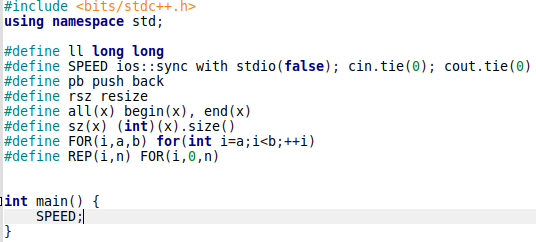
\includegraphics[scale=0.4]{template}

\section{Data Structures}
\subsection{Segment Tree}

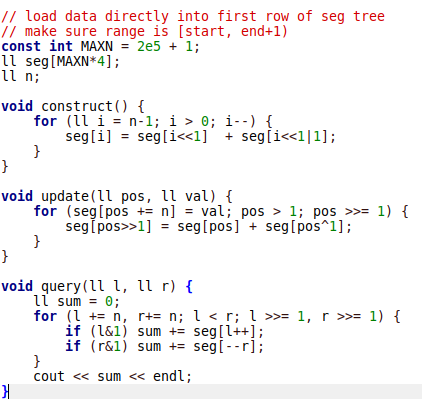
\includegraphics[scale=0.4]{segmenttree}

\subsection{Minimum Sparse}

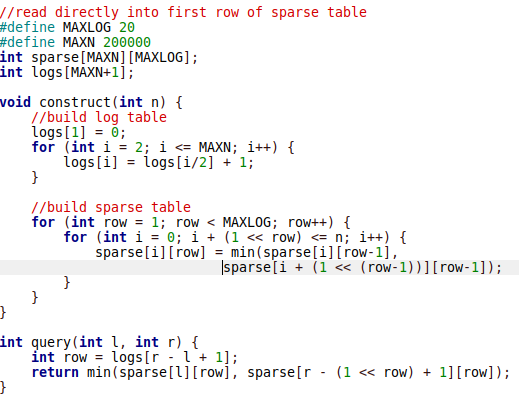
\includegraphics[scale=0.4]{sparsemin}

\subsection{Binary Jumping}

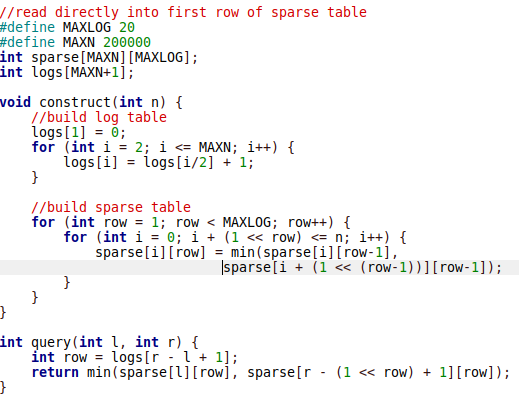
\includegraphics[scale=0.4]{sparsemin}

\section{Graph Algorithms}
\subsection{DFS with Cycle Detection}
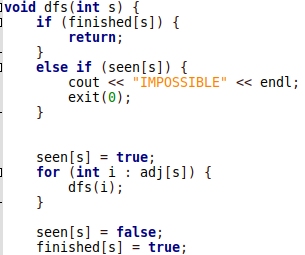
\includegraphics[scale=0.5]{dfs}
\subsection{BFS}
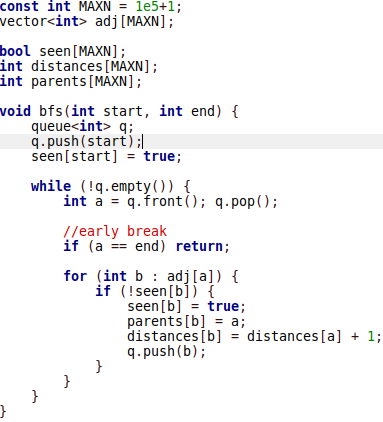
\includegraphics[scale=0.5]{bfs}
\subsection{BFS Route Reconstruction}
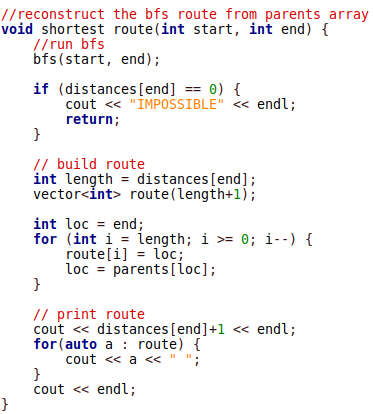
\includegraphics[scale=0.5]{bfsroutes}
\subsection{Djikstra}
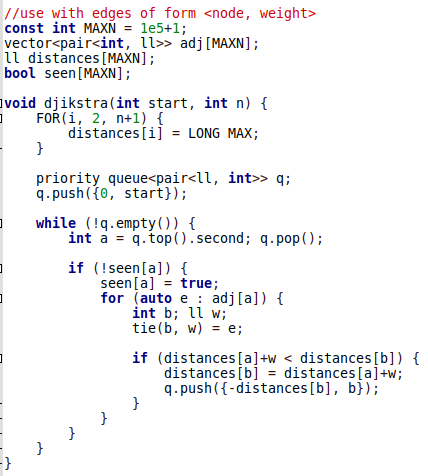
\includegraphics[scale=0.5]{djikstra}
\subsection{Bellman-Ford}
\subsection{Floyd-Warshall}
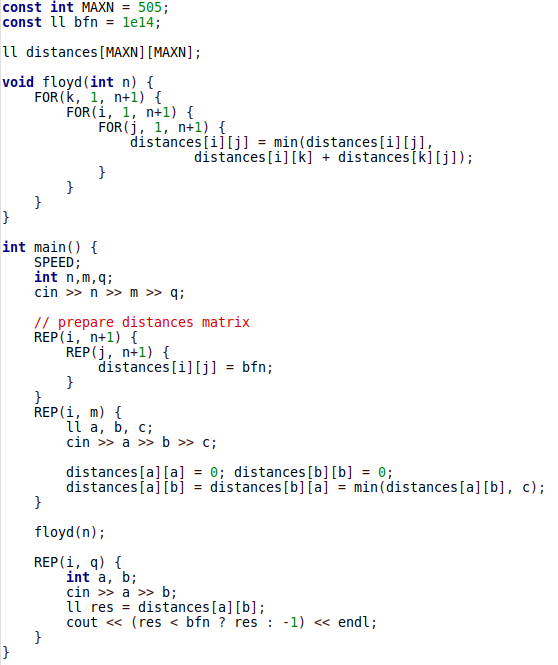
\includegraphics[scale=0.4]{floyd}
\subsection{Topological Sort}
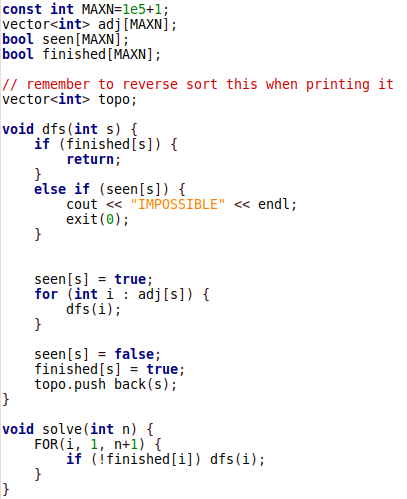
\includegraphics[scale=0.5]{topological}
\subsection{Kruskal with DSU}
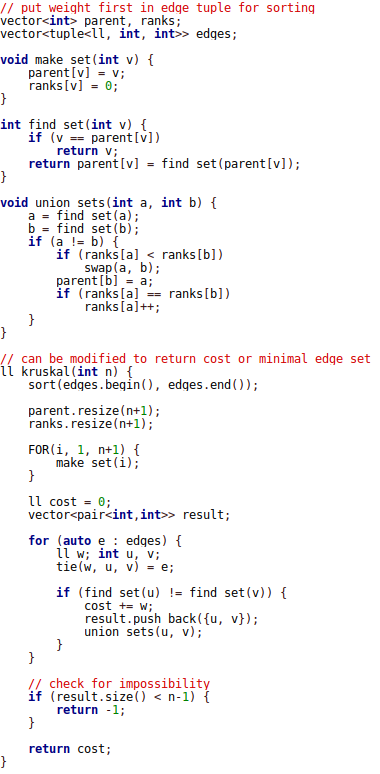
\includegraphics[scale=0.5]{kruskal}

\subsection{Connected Components}
For counting, use DFS and increment whenever the recursive call is completely finished. For listing, keep a vector that gets appended to during DFS. Print the vector, then reset it for the next component.

\section{Dynamic Programming}
\subsection{Longest Increasing Subseqeuence}

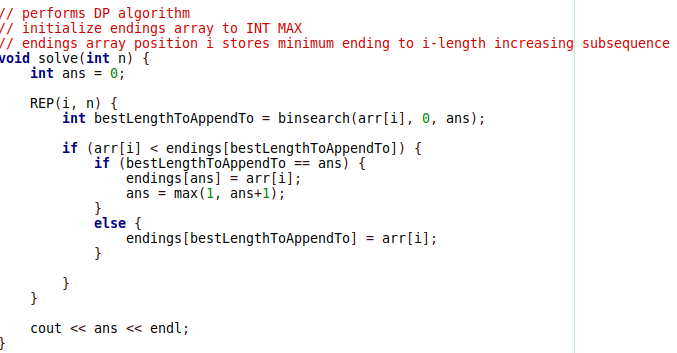
\includegraphics[scale=0.5]{lis}

\subsection{Edit Distance}
\subsection{Coins Problem}
\subsection{Knapsack}
\subsection{Rod Cutting}


\section{Miscellaneous}
\subsection{Binary Search}

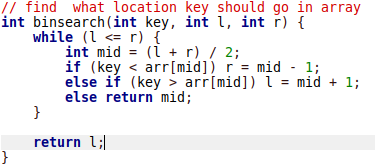
\includegraphics[scale=0.5]{binsearch}

\subsection{Binary Exponentiation}

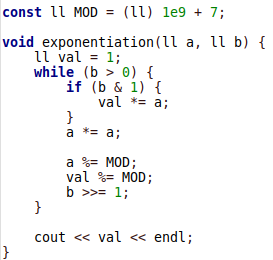
\includegraphics[scale=0.5]{binexp}

\subsection{Gray Code}

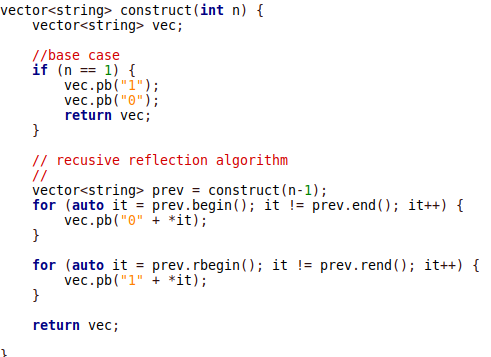
\includegraphics[scale=0.5]{graycode}

\subsection{Towers of Hanoi}
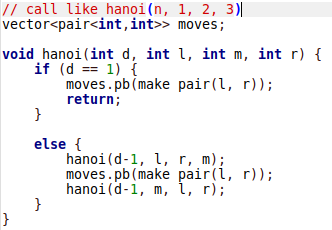
\includegraphics[scale=0.5]{hanoi}

\subsection{Josephus Queries}
O(n)

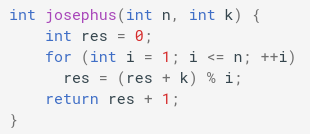
\includegraphics[scale=0.5]{josephus}

O(klogn)

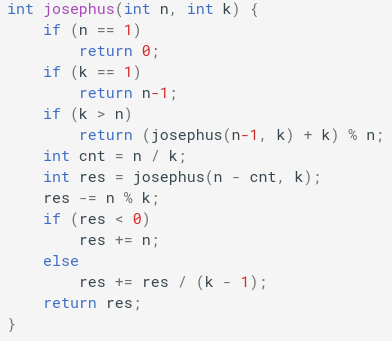
\includegraphics[scale=0.5]{quickjosephus}
\end{document}
